\documentclass{beamer}
%\usetheme{Boadilla}
%\usetheme[height=7mm]{Rochester}
\usetheme{Warsaw} 
\setbeamertemplate{items}[ball]
%\setbeamertemplate{blocks}[rounded][shadow=true] 
\setbeamertemplate{navigation symbols}{} 

\usepackage{tikz}
%\usetikzlibrary{arrows,decorations.pathmorphing,backgrounds,placments,fit}
\usetikzlibrary{%
  arrows,%
  shapes,%
  chains,%
  matrix,%
  positioning,% wg. " of "
  scopes,%
  decorations.pathmorphing,% /pgf/decoration/random steps | erste Graphik
  shadows%
}

\tikzstyle{every picture}+=[remember picture]
% By default all math in TikZ nodes are set in inline mode. Change this to
% displaystyle so that we don't get small fractions.
\everymath{\displaystyle}

\usepackage{pgfplots}

\pgfdeclarelayer{background}
\pgfdeclarelayer{foreground}
\pgfsetlayers{background,main,foreground}

%%%%%%%%%%%%%%%%%%%%%%%%%%%%%%%%%%%%%%%%%%%%%%%%%%%%%%%%%%%%%%%%%%
%% Useful macros for equations

\newcommand{\pow}{\ensuremath{\wedge} }
\newcommand{\poweq}{\ensuremath{\wedge =} }

\newcommand{\deriv}[2]{\ensuremath{\frac{\partial #1}{\partial #2}}}
\newcommand{\dderiv}[2]{\ensuremath{\frac{\partial^2 #1}{\partial {#2}^2}}}
\newcommand{\Vpar}{\ensuremath{V_{||}}}
\newcommand{\Gradpar}{\ensuremath{\partial_{||}}}
\newcommand{\Divpar}{\ensuremath{\nabla_{||}}}
\newcommand{\DivXgradX}[2]{\ensuremath{\nabla_\psi\left(#1\partial_\psi #2\right)}}
\newcommand{\DivParGradPar}[2]{\ensuremath{\nabla_{||}\left(#1\partial_{||} #2\right)}}

\newcommand{\apar}{\ensuremath{A_{||}}}
\newcommand{\hthe}{\ensuremath{h_\theta}}
\newcommand{\Bp}{\ensuremath{B_\theta}}
\newcommand{\Bt}{\ensuremath{B_\zeta}}

\newcommand{\bvec}{\mathbf{b}}
\newcommand{\kvec}{\mathbf{\kappa}}
\newcommand{\bxk}{\bvec_0\times\kvec_0\cdot\nabla}
\newcommand{\Bvec}{\mathbf{B}}
\newcommand{\Bbar}{\overline{B}}
\newcommand{\Lbar}{\overline{L}}
\newcommand{\Tbar}{\overline{T}}
\newcommand{\Jvec}{\mathbf{J}}
\newcommand{\Jpar}{J_{||}}
\newcommand{\Apar}{A_{||}}
\newcommand{\delp}{\nabla_\perp^2}
\newcommand{\Div}[1]{\ensuremath{\nabla\cdot #1 }}
\newcommand{\Curl}[1]{\ensuremath{\nabla\times #1 }}
\newcommand{\rbp}{\ensuremath{R\Bp}}
\newcommand{\rbpsq}{\ensuremath{\left(\rbp\right)^2}}
\newcommand{\noun}[1]{\textsc{#1}}
\newcommand{\vE}{\ensuremath{\mathbf{v}_E}}
\newcommand{\vort}{\ensuremath{\overline{\omega}}}

%%%%%%%%%%%%%%%%%%%%%%%%%%%%%%%%%%%%%%%%%%%%%%%%%%%%%%%%%%%%%%%%%%

\begin{document}

\title[Introduction to BOUT++ (\insertframenumber\ of \inserttotalframenumber)]{Introduction to BOUT++}
\author{Ben Dudson\\
\texttt{benjamin.dudson@york.ac.uk}}

\pgfdeclareimage[width=0.5\textwidth]{yorklogo}{york_logo.png} 
\pgfdeclareimage[width=0.4\textwidth]{llnllogo}{llnl_logo.png}
\institute[Uni. York]{Department of Physics, University of York, Heslington, York YO10 5DD, UK}
\date{LLNL, 14$^{th}$ September 2011\\
\pgfuseimage{yorklogo}\\
\pgfuseimage{llnllogo} \hspace{0.05\textwidth}}
\begin{frame}
\titlepage
\end{frame}

\begin{frame}
  \frametitle{The BOUT++ code}
  
  \begin{itemize}
    \item Plasma fluid simulation framework\footnote{B.D.Dudson et. al. Comp. Phys. Comm. 180 (2009), pp. 1467-1480}
    \item Solves an arbitrary number of fluid equations in curvilinear coordinates
    \item Finite difference with implicit or explicit timestepping.
      Methods can be changed at run-time, and include 4th-order Central differencing, Arakawa, and 3rd-order WENO.
    \item Written in C++, open source (LGPL)\footnote{Available at \texttt{http://github.com/bendudson/BOUT}}
  \end{itemize}

  \includegraphics[width=0.3\textwidth]{lapd_slice.pdf}
  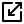
\includegraphics[width=0.35\textwidth]{scaling.pdf}
  \includegraphics[width=0.29\textwidth]{ptot_44_sm.pdf}
\end{frame}

\begin{frame}
  \frametitle{What is BOUT++}
  
  \begin{itemize}
  \item Framework for writing fluid / plasma simulations in curvilinear geometry
  \item Finite-difference code, variety of numerical methods and time-integration solvers
  \item Written from scratch in C++, borrowing some ideas from the original
    BOUT code
  \item Intended to be quite modular, enabling fast testing of numerical methods
  \item Can evolve any number of equations, with equations appearing in a readable form
  \item Primarily designed and tested with reduced plasma fluid models in mind
  \end{itemize}
  
\end{frame}

\begin{frame}
  \frametitle{What {\bf isn't} BOUT++}
  
  \begin{itemize}
  \item Not a general parallel simulation library. Better tools such as PETSc
    exist for that
  \item Not a magic bullet. It doesn't automate the process of choosing an appropriate numerical scheme, just makes it easier to implement and test different ones
  \item Not suitable for every problem. The numerical methods currently implemented are quite general, but cannot cover all problems
  \end{itemize}
\end{frame}

\begin{frame}
  \frametitle{Overall aims}
  
  \begin{itemize}
  \item Started with the aim of simulating ELMs. Appropriate physics model
    not known. Wanted to make the code easy to change
  \item Large codes often hard to understand, so wanted to isolate the
    model-specific code into a small number of lines
  \item Still hard to understand whole code, but clearer what problem is being solved
  \end{itemize}

  \pause
  
  Now becoming more widely used, and aim is to build a 
  community to use and develop the code further
  
  Separated into model-specific and general code, so we can
  \begin{itemize}
  \item  Work on multiple different physics problems separately
  \item  Benefit from each other's improvements to the core code
  \end{itemize}
\end{frame}

\begin{frame}[fragile]
  \frametitle{Status and capabilities}
  \begin{itemize}
  \item Equations appear in a form which is (reasonably) clear e.g.
    \begin{verbatim}
      ddt(Apar) = - Grad_par(phi);
    \end{verbatim}
    \vspace{-0.5cm}
  \item Can simulate a variety of fluid models. Mainly subsets of
    Braginskii, but also full MHD and compressible gas equations
    \pause
  \item Usually uses a field-aligned Clebsch coordinate system, but
    most operators are general. Only needs the metric tensor components
    to be specified.
    \pause
  \item Contains a library of different numerical differencing methods,
    and time-integration schemes. Simple schemes built-in, but uses
    external libraries such as SUNDIALS and PETSc for advanced methods
    \pause
  \item Promising results for turbulence and ELM simulations. Xu
    will talk more about this next...
  \item For typical ELM simulations the code scales well to
    a few thousand cores
  \end{itemize}
\end{frame}

\begin{frame}
  \frametitle{Work in progress}
  
  \begin{itemize}
  \item Coupling to the PETSc library for time-stepping working and under
    development
  \item Gyro-fluid extensions (gyro-averaging operators) working and
    being tested
  \item Pre-processing routines to prepare equilibria functional, but 
    needs improvement
  \item Test cases: many example problems, and some unit tests. More needed to
    allow regular regression testing
  \item Documentation. Quite extensive manuals, but lags behind code
  \end{itemize}
\end{frame}

\begin{frame}
  \frametitle{Future developments}
  
  \begin{itemize}
  \item Preconditioning methods, including physics-based
  \item More advanced numerical methods, both differencing and time-integration
  \item Improved handling of highly non-uniform meshes
  \item Additional differential operators to model effects like Landau damping
  \item Coupling to external databases or codes to model things like atomic
    physics, fuelling and interactions with core and walls
  \item Better visualisation tools, in languages other than IDL
  \item Use of external libraries (e.g. PETSc, hypre) for 
    linear and nonlinear solvers
  \item Scalability beyond 10,000 cores 
  \end{itemize}
\end{frame}

\begin{frame}
  \frametitle{Access to BOUT++}
  
  The BOUT++ code is open source, and publically available at github.com

  \begin{block}
    
    \begin{center}
      http://github.com/bendudson/BOUT
    \end{center}
  \end{block}
  
  For this workshop, we have created a ``stable'' version 1.0, which may be
  updated with bugfixes, but no new features
  
  \begin{block}
    
    \begin{center}
      http://github.com/bendudson/BOUT-1.0
    \end{center}
  \end{block}
  
  Anyone can download a copy, but to make changes you will need to set up
  an account and SSH keys on github. Sean Farley will cover this after coffee...
\end{frame}

\begin{frame}
  \frametitle{Why use Git?}
  
  \begin{itemize}
  \item Git was written by Linus Torvalds with Linux development in mind, so
    can easily handle very large collaborations and complicated merging
  \item Doesn't enforce any particular way of working, and doesn't have
    the concept of a ``central'' server - all copies of the code are equivalent
  \item A particular copy of BOUT++ is only ``the'' version by consent (or diktat)
  \end{itemize}
  
  This can seem strange coming from SVN, but makes it easier to work
  independently on features, then merge changes together afterwards.
  
  $\Rightarrow$ Hopefully a help, rather than a hinderance to collaboration
\end{frame}

\begin{frame}
  \frametitle{Use of BOUT++}
  
  Contributing:
  \begin{itemize}
  \item BOUT++ is under the LGPL license, so code which uses it can be proprietry. Modifications to the BOUT++ library do come under the LGPL
  \item You're free to take and modify BOUT++ for any purpose
  \item We would appreciate it if you contributed back improvements
    you make to the code
  \end{itemize}
  
  \pause
  
  Support:
  \begin{itemize}
  \item We're happy to help, but our time is limited
  \item One aim of this workshop is to get a group of people comfortable with
    using BOUT++ and (eventually) help support each other
  \item There is a BOUT++ development mailing list. Please let me know 
    if you'd like to join it
  \end{itemize}
\end{frame}

\begin{frame}
  \frametitle{Summary}
  
  \begin{itemize}
  \item BOUT++ is a fluid simulation framework designed with plasma edge
    simulations in mind
  \item Less general than libraries like PETSc, still very flexible for plasma
    applications
  \item A tool to speed up development of new plasma models and numerical methods
    \pause
    \vspace{1cm}
  \item Not perfect... \\
    I look forward to working with you to improve it
  \end{itemize}
 
\end{frame}

\end{document}
